%%%%%%%%%%%%%%%%%%%%%%%%%%%%%%%%%%%%%%%%%%%%%%%%%%%%%%%%%%%%%%%%%%%%%%%%%%%
%%%                                                                     %%%
%%%   LaTeX template voor het verslag van P&O: Computerwetenschappen.   %%%
%%%                                                                     %%%
%%%   Opties:                                                           %%%
%%%     tt      Tussentijdsverslag                                      %%%
%%%     eind    Eindverslag                                             %%%
%%%                                                                     %%%
%%%   4 november 2013                                                   %%%
%%%   Versie 1.1                                                        %%%
%%%                                                                     %%%
%%%%%%%%%%%%%%%%%%%%%%%%%%%%%%%%%%%%%%%%%%%%%%%%%%%%%%%%%%%%%%%%%%%%%%%%%%%

\documentclass[eind]{penoverslag}

%%% PACKAGES %%%
\usepackage{graphicx}
\usepackage{amsmath}
\usepackage{wasysym}
\usepackage{float}
\usepackage{wrapfig}
\setlength\parindent{0pt}

\begin{document}

% == TITELPAGINA == %
\team{Indigo} % teamkleur
\members{\\
        Wander Bavin\\
        Vince Goossens\\
        Dimitri Jonckers\\
        Sunil Tandan\\
				Wout Vekemans} % teamleden				
\maketitlepage


% == SAMENVATTING == %
\begin{abstract}
\noindent
Dit rapport documenteert onze analyse en oplossing van het volgende probleem : een zeppelin die aangestuurd wordt door een Raspberry Pi, gemonteerd aan een frame met 3 motoren en   gelift door 2 grote ballonnen, moet opdrachten kunnen uitvoeren. Deze opdrachten, die via QR-codes worden meegegeven, moeten autonoom door de zeppelin worden uitgevoerd. Het uiteindelijke doel is om zo een traject af te leggen dat door de commando's wordt bepaald. Hiervoor hebben we Java-software ontwikkeld die op de Pi draait. Deze regelt de motoren en verwerkt de commando's. Ook kan de gebruiker via een GUI op de client-pc kiezen voor manuele of automatische besturing en de status van de zeppelin bekijken. \\

!!!!!Todo : 2 zinnen over besluit (wat werkt)!!!!!!!!!!!
\end{abstract}


% == INHOUDSOPGAVE == %
\tableofcontents\newpage


% == INLEIDING == %
\section{Inleiding}
Het doel van deze opdracht is een autonome zeppelin te ontwikkelen. De zeppelin wordt aangestuurd door een Raspberry Pi. Via QR-codes kunnen instructies gegeven worden, zoals ``stijg 50 cm'' of ``draai 45   graden''. De gebruiker kan via een GUI op een client-pc zelf de pijltjestoetsen gebruiken om de zeppelin aan te sturen of gegevens bekijken over de toestand van de zeppelin (bijvoorbeeld de huidige hoogte).

\paragraph{Fysisch ontwerp}
~\\ 
De zeppelin bestaat uit een houten frame waaraan 2 heliumballonnen ($\diameter$90 cm) vastgemaakt zijn. Aan het frame zijn een camera en een afstandssensor vastgemaakt, die beiden naar beneden gericht zijn. Zowel de camera als de afstandssensor zijn verbonden met de Raspberry Pi die in het frame zit ingebed. Het geheel bevat drie propellers: twee voor horizontale bewegingen en \'{e}\'{e}n voor verticale bewegingen.


\paragraph{Software ontwerp}
~\\
Het grootste deel van de opdracht is het schrijven van de software in een taal naar keuze. Wij hebben gekozen voor Java. De software bestaat uit 3 grote delen: de GUI, de communicatie tussen GUI en Raspberry Pi en de interne programmatie op de Pi (Zie figuur \ref{schema}). \\
De communicatie tussen GUI en de Raspberry Pi gebeurt via sockets. Hierbij worden objecten uitgewisseld tussen de client en de server (de Pi), die commando's doorgeven aan de zeppelin of de status doorgeven aan de gebruiker. De interne programmatie op de Pi moet op basis van gegevens van zijn sensoren en instructies van QR-codes (en commando's van de gebruiker) de motoren aansturen. 

\begin{figure}[ht!]
\centering
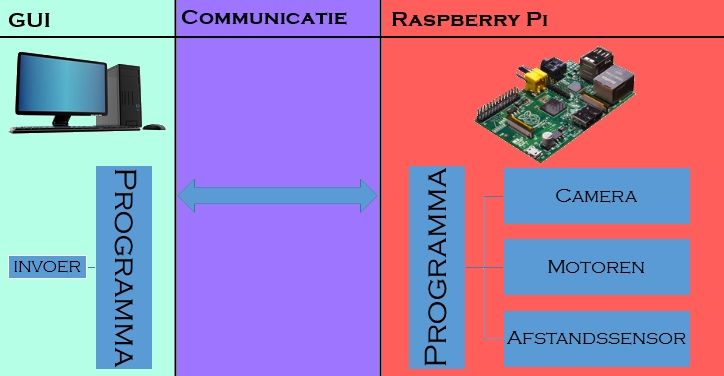
\includegraphics[height=55mm]{Schema.jpg}
\caption{Architectuur}
\label{schema}
\end{figure}

\newpage

% == Beschrijving materiaal en bouw zeppelin == %
\section{Beschrijving materiaal en bouw zeppelin}
De zeppelin bestaat uit een frame waaraan alle onderdelen zijn vastgemaakt. Hierop worden onder andere 3 propellers bevestigd. Twee hiervan dienen om naar links en rechts te draaien. Om vooruit te bewegen worden deze samen geactiveerd met dezelfde kracht. Deze propellers bevinden zich aan de uiteindes van de vleugels. De derde propeller, om de zeppelin te laten stijgen, is naar beneden gericht. De propellers kunnen op volle kracht of door middel van pwm\footnote{en.wikipedia.org/wiki/Pulse-width\_modulation}  worden aangestuurd (in 2 richtingen). Met deze techniek is het mogelijk om naast de richting ook de kracht van de motor in te stellen.~\\

\begin{figure}[h!]
\centering
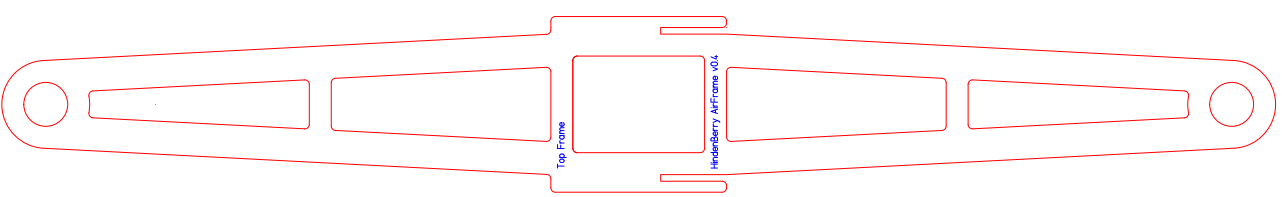
\includegraphics[scale=0.3]{upperFrame.png}
\label{frame}
\end{figure}

\begin{figure}[h!]
\centering
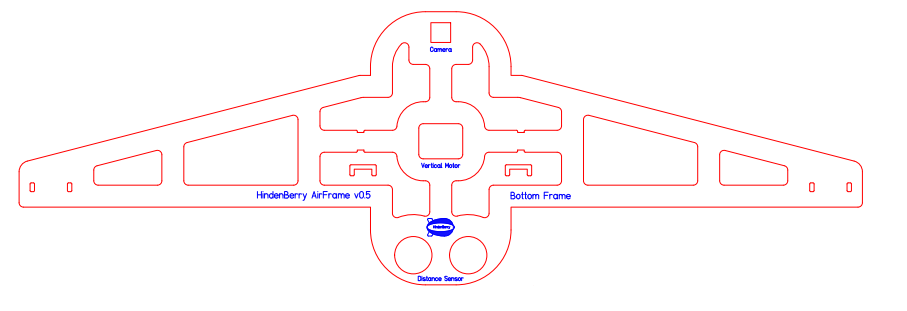
\includegraphics[scale=0.3]{lowerFrame.png}
\caption{Blueprint van het frame}
\label{frame}
\end{figure}

Om het geheel in de lucht te houden, zitten er 2 heliumballonnen ($\diameter$90 cm) vast aan de bovenkant van het frame. Deze hebben initieel een lift van 268 gr per stuk, maar dit vermindert wanneer de ballonnen doorheen de weken volume verliezen. \\

De zeppelin wordt aangestuurd door een Raspberry Pi model A. Deze heeft volgende specificaties: 
\begin{itemize}
	\item \emph{Processor:} 700MHz ARM
	\item \emph{Geheugen:} 256MB 
	\item \emph{Poorten:} 1 USB 2.0, HDMI, audio out, RCA video
	\item \emph{Voeding:} Micro USB
	\item GPIO-pinnen om de hardware aan te sturen
\end{itemize}

In de Raspberry Pi zit een SD-kaart van 4 GB. Hierop staat Raspbian, het standaard besturingssysteem van de Raspberry Pi. \\

Verder zijn er nog 2 devices waarvan de zeppelin gebruik maakt:
\begin{itemize}
	\item \emph{De camera} laat toe foto's te nemen met een maximum resolutie van 5 MP. Hiermee kunnen we onder andere beelden maken van QR-codes. Daarnaast kan de camera video's maken met resoluties tot 1080p. 
	\item \emph{De afstandssensor} kan worden gebruikt om met ultrasone trillingen de afstand te meten tussen de zeppelin en de grond of muur. Het bereik gaat van 2-400 cm. \\
\end{itemize}

\begin{figure}[ht!]
\centering
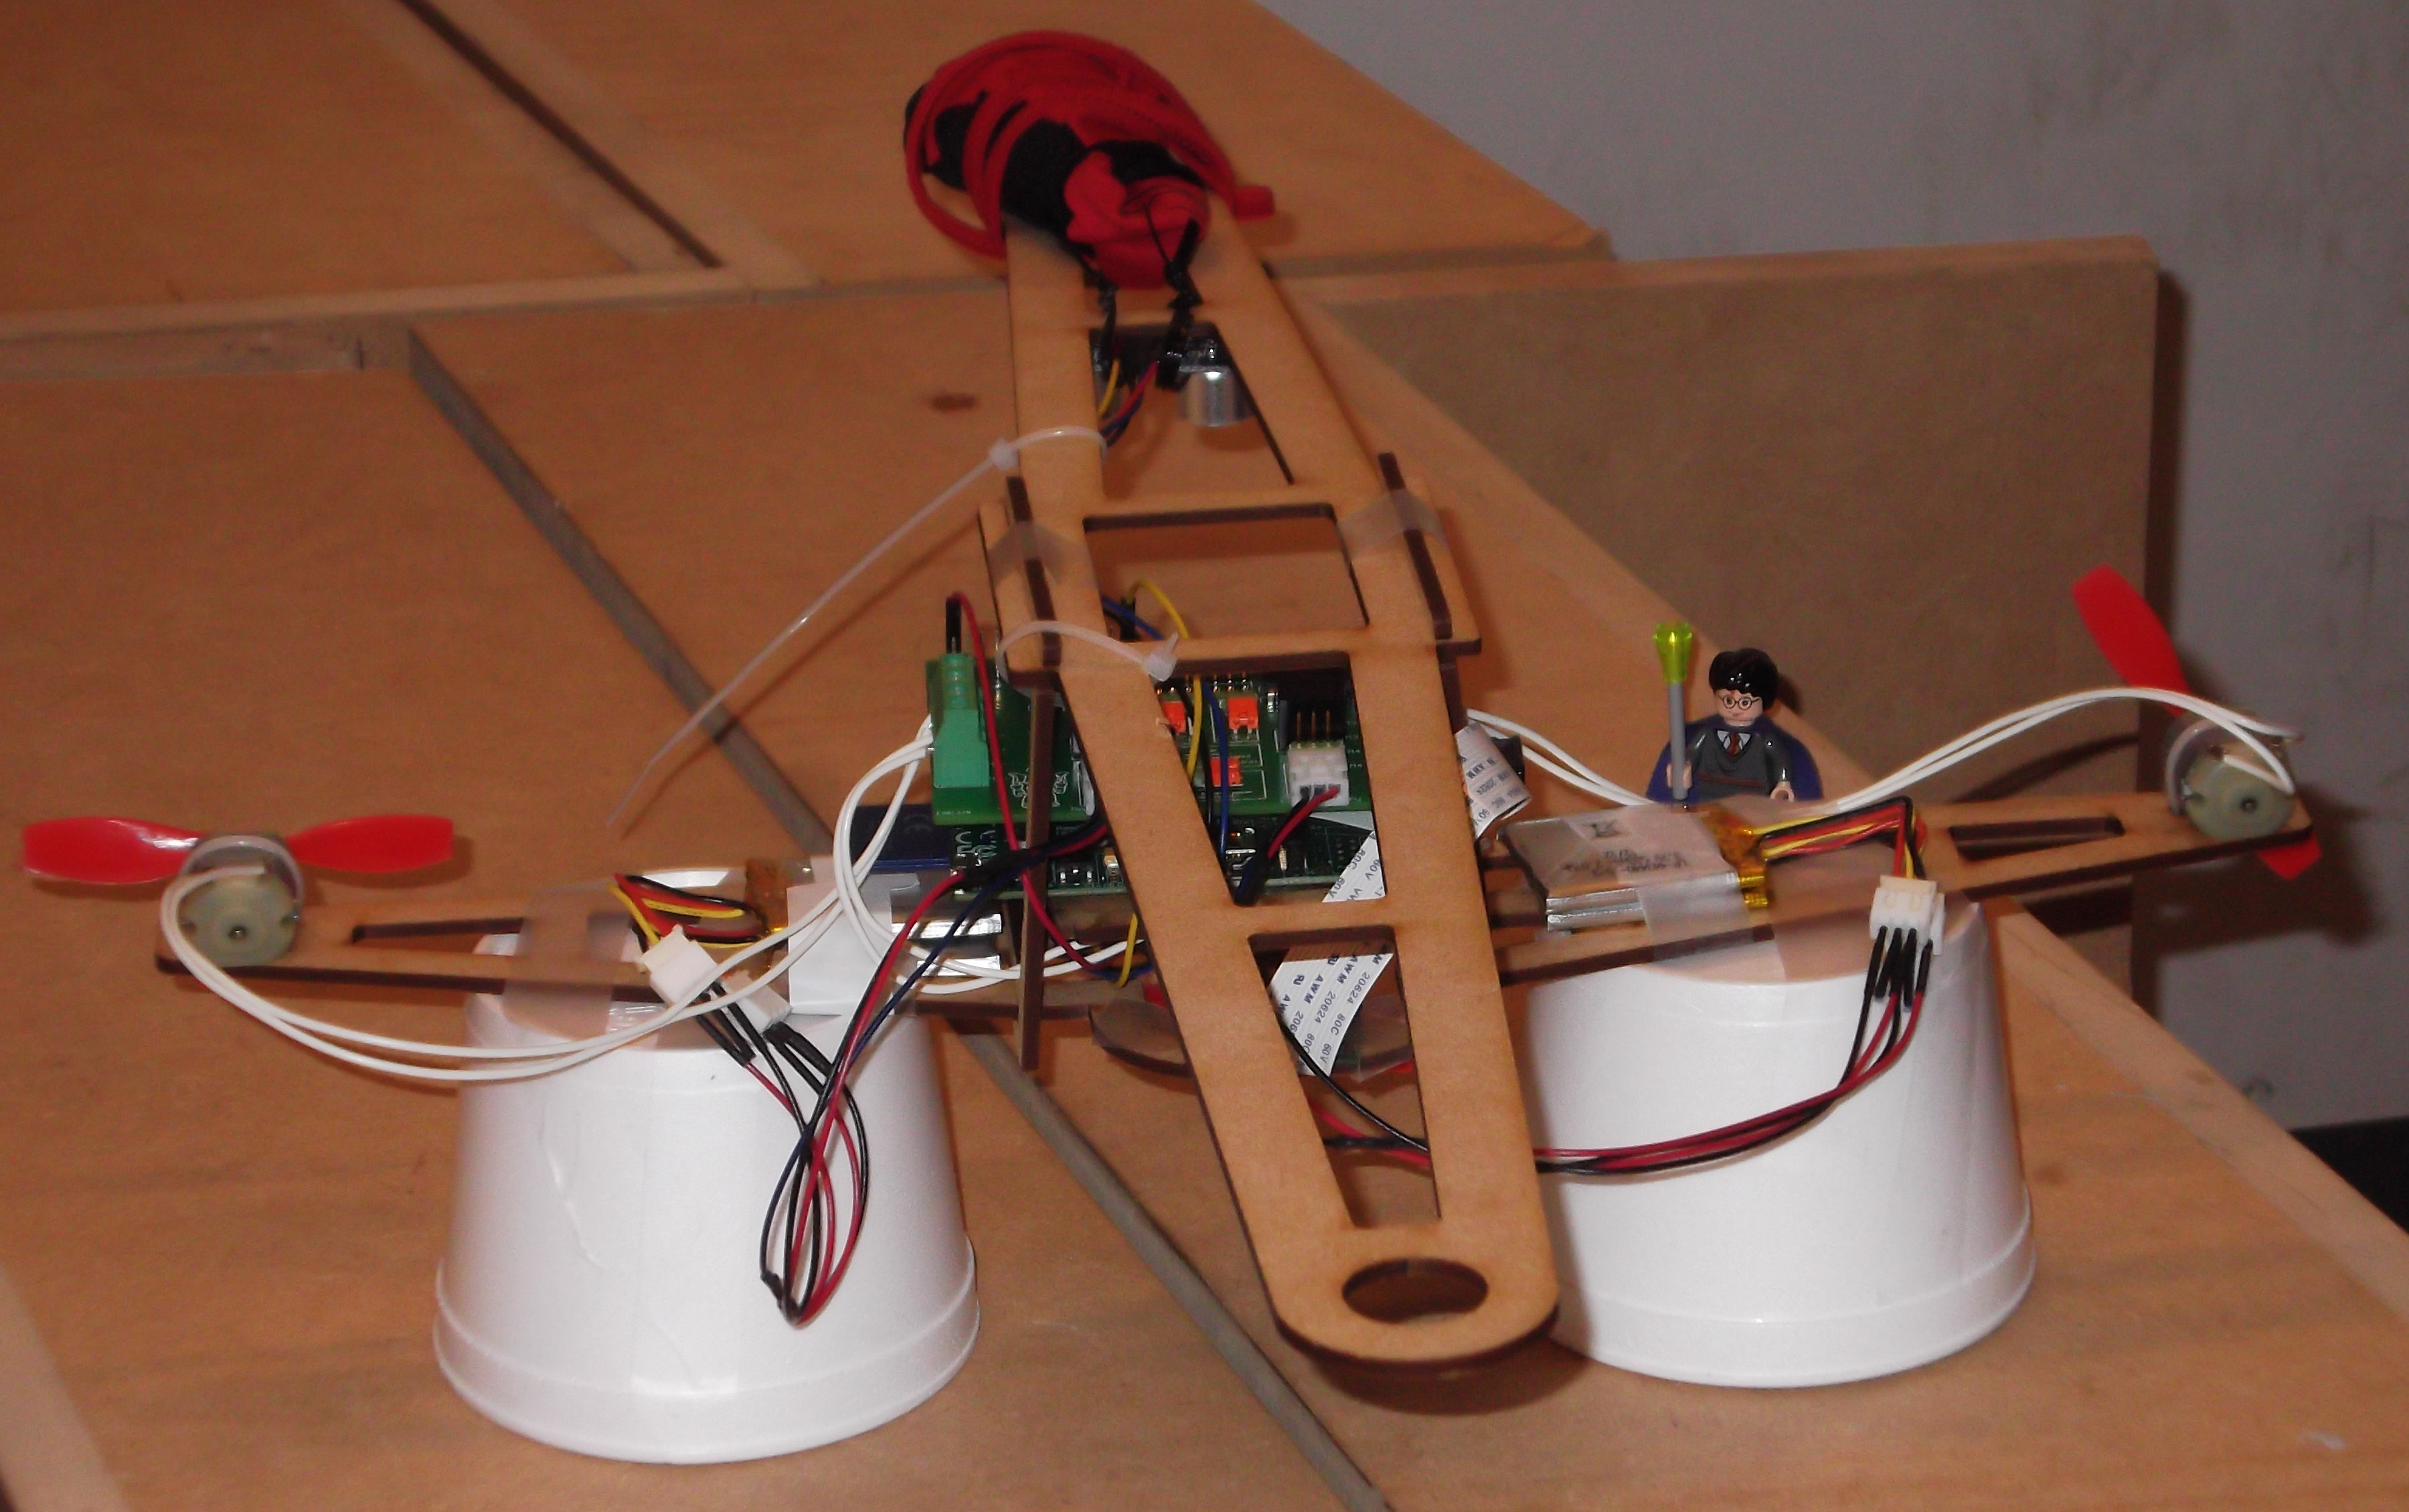
\includegraphics[height=60mm]{zeppelinFrame.jpg}
\caption{Frame met gemonteerde onderdelen}
\label{zeppFrame}
\end{figure}

Om het geheel te monteren, hebben we gebruik gemaakt van plakband en zipties (bundelbandjes). We hebben bekertjes bevestigd om ballast te dragen, zodat het geheel lichtjes zakt wanneer de motor geen kracht naar boven zet. Als gewicht gebruiken we zout, zodat het mogelijk is om nauwkeurig het gewicht te regelen. \\

% == Testen == %
\section{Testen}

Om er zeker van te kunnen zijn dat het aansturen van de zeppelin correct gebeurt, is het nodig dat de componenten getest worden. In deze sectie volgt hierover meer informatie. \\
\subsection{Afstandssensor}

In dit deel gaan we dieper in op de testen die we gedaan hebben naar de nauwkeurigheid en snelheid van de afstandssensor.

\paragraph{Opstelling} ~\\ 
Benodigdheden:
\begin{itemize}
	\item RaspberryPi met afstandssensor
	\item houten scherm
	\item meetlat
\end{itemize}
Deze componenten worden in deze opstelling geplaatst : zie figuur \ref{opstelling}

\begin{figure}[ht!]%
\centering
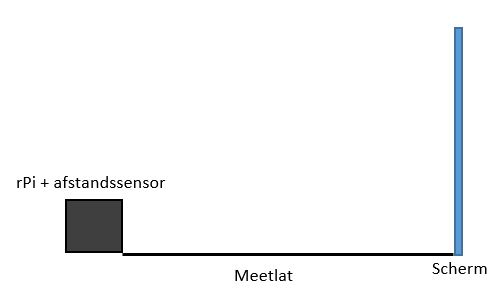
\includegraphics[scale=0.6]{opstelling.jpg}%
\caption{testopsteling}%
\label{opstelling}%
\end{figure}

\paragraph{Verloop} ~\\ 
De test bestaat uit het meten van 11 verschillende afstanden (10, 20, 30, 60, 90, 100, 110, 120, 130, 140 en 150 cm). Deze zijn zo gekozen om informatie te hebben over voldoende punten binnen het vlieghoogtebereik. Deze afstanden worden elk 500 keer gemeten, om de 60 ms. Deze waarden zijn zo gekozen, om toch voldoende nauwkeurigheid te hebben, veronderstellende dat er uitschieters zouden zijn.

\paragraph{Gegevens en verwerking} ~\\ 
We hebben d.m.v. rolling median de mediaan berekend van 10 en 20 opeenvolgende gegevens, uit de set van 500 waardes per hoogte. Minder dan 10 is niet nauwkeurig genoeg en voor meer dan 20 samples is de registratietijd te hoog. Uit deze gegevens hebben we om een aantal redenen besloten om een window van 10 samples te nemen.  Ten eerste is er de nauwkeurigheid als de zeppelin stijgt/daalt. Het hoogteverschil tussen sample 1 en 10 is immers kleiner dan dat tussen 1 en 20. Ten tweede is er de snelheid. Het spreekt voor zich dat het registreren van 10 samples minder lang duurt dan 20 samples. Tenslotte is er ook het minieme verschil tussen de gemiddelde mediaan bij 10 en 20 metingen. Minder metingen zorgen dus voor een quasi-gelijke nauwkeurigheid. 

Een nadeel is wel dat de standaardafwijking van de medianen bij een breedte van 10 samples gemiddeld 0.2 cm groter is dan bij 20 samples. Dit weegt echter niet op tegen de winst aan snelheid en nauwkeurigheid.\\ 

Voor de meetgegevens: zie Tabel 1. \\
\begin{table}
\begin{tabular}{r||r|r|r|r|r|r|r|r|r|r|r}
\textbf{Afstand} & 10 & 20 & 30 & 60 & 90 & 100 & 110 & 120 & 130 & 140 & 150 \\
\hline \hline 
$\mu$ (med.) (10) & 10.8 & 20.5 & 30.8 & 58.0 & 88.3 & 98.7 & 108.5 & 117.3 & 127.74 & 137.0 & 147.10 \\
$\mu$ (med.) (20) & 10.8 & 20.7 & 30.7 & 58.0 & 88.3 & 98.7 & 108.5 & 117.3 & 127.7 & 137.0 & 147.1 \\
$\sigma$ (med.) (10) & 0.21 & 0.52 & 0.82 & 0.55 & 0.70 & 0.72 & 0.68 & 0.94 & 0.58 & 0.60 & 0.69 \\
$\sigma$ (med.) (20)& 0.09 & 0.33 & 0.71 & 0.41 & 0.59 & 0.56 & 0.47 & 0.54 & 0.43 & 0.37 & 0.49 \\
\end{tabular}
\emph{\caption{Gemiddelde en standaardafwijking van de rolling medians van 10 en 20, uit 500 meetwaarden}}
\label{tab:Meting}
\end{table}

Het uitvoeren van de testen nam per afstand gemiddeld 32 seconden in beslag. Omdat dit tijdens het opereren van de zeppelin veel te lang is, hebben we besloten om de tijd tussen de metingen te verkorten. Zo kunnen de metingen sneller gebeuren. Hiervoor hebben we een extra test uitgevoerd op een hoogte van 170cm en 200cm (kleiner interval zou voor interferentie kunnen zorgen op grote afstanden). Het blijkt dat we het interval tussen metingen kunnen terugbrengen naar 20 ms. Bij lagere waardes gaan de signalen door elkaar lopen en dit kan de meting verstoren. \\

\paragraph{Conclusie} ~\\ 
De afstandsmeter meet het meest nauwkeurig bij kleine afstanden, bij grotere afstanden (meer dan 60 cm) liggen de meetresultaten gemiddeld iets onder de werkelijke afstand. Relatief gezien blijft de fout nog klein en kunnen we deze afwijking in het vervolg incalculeren bij het bepalen van de meetwaarden. De afstandssensor geeft telkens de mediaan van 10 gegevens door volgens het principe van de “rolling median”-techniek. Tien gegevens zorgen voor voldoende nauwkeurigheid, maar hebben ook het aspect dat de mediaanberekeningen snel genoeg gebeuren. Tevens is dit bij een hoogteverandering accurater. Deze methode boet wel in op de standaardafwijking. De gegevens wijken dus meer uit, maar dit weegt niet op tegen de voorgenoemde pluspunten. Om de afstandsregistratie nog sneller te laten verlopen, meet de afstandsmeter om de 20 ms.

\subsection{Camera en QR-code parser}
De camera moet in staat zijn om foto's te nemen en de QR-code te herkennen. De focus bij het testen lag op resolutie, responstijd van de camera, positie van de QR-code op de foto en invalshoek. \\

We hebben testen uitgevoerd waarin de QR-code lichtjes gedraaid was (invalshoek). Dit hebben we uitgevoerd tot hoeken van 20 graden, en er was geen probleem om ze te lezen. \\

Daarna hebben gezocht naar een geschikte resolutie waarbij de QR-code gelezen kan worden. Voor een afstand van 2 meter is een resolutie van 600 x 800 pixels nodig. Bij afstanden kleiner dan of gelijk aan 1.20 m kunnen we dit verlagen tot 400 x 600 pixels. \\

De responstijd (tijd tot herkennen QR-code) is getest door in verschillende omstandigheden een code te fotograferen. Een simpel printcommando in Java vertelt ons hoe lang het nemen van de foto en het verwerken duurt. Hiervoor wordt de interne klok van de computer gebruikt. Om een globaal beeld te krijgen van de responstijd wordt een gemiddelde berekend van deze gegevens. Een hogere resolutie zorgt voor een langere verwerkingstijd. Bij een resolutie van 600 x 800 duurt het lezen gemiddeld 6 seconden, met een maximum van 8 seconden. Bij een resolutie van 400 x 600 duurt het lezen gemiddeld 3.5 seconden. \\

De positie van de QR-code blijkt geen problemen op te leveren voor het lezen van de QR-code. Hiervoor hebben we de QR-code op verschillende plaatsen (weg van het midden) binnen het beeld gezet.\\ %De codes bevatten commando’s die relatief ten opzichte van de huidige positie moeten worden uitgevoerd.%

Het is wel duidelijk geworden dat meerdere QR-codes binnen een beeld (soms) een probleem opleveren. Wanneer ze dichter dan 10 cm bij elkaar staan, slaagt de parser er niet meer in ze te interpreteren. Indien dit zich voordoet, zullen we moeten zakken, een nieuwe foto nemen en terug naar de oorspronkelijke hoogte gaan. \\

\paragraph{Conclusie} ~\\
We kunnen stellen dat de camera en QR-parser in de meeste gevallen geen problemen opleveren. De resolutie passen we aan op basis van de hoogte: bij hoogtes lager dan 1.20 m nemen we 400 x 600, anders nemen we 600 x 800. \\


\subsection{Motoren}
Eerste experimenten focusten op de kracht van de motoren en op het aan de praat krijgen van de pwm. De documentatie van onze library voor het aansturen van de pinnen was hierover niet heel duidelijk, maar we hebben gemerkt dat we pwm-waardes tussen 0 en 1024 kunnen opgeven. Een minimale pwm-waarde van ongeveer 740 is nodig om de propeller in beweging te krijgen. \\

Vervolgens zijn we begonnen met het testen voor verticale bewegingen (up-motor). Dit was nodig om de hoogte te regelen, hetgeen voor de eerste demonstratie in orde moest zijn. De horizontale bewegingen volgden later. \\

In wat volgt beschrijven we testen van de motoren zelf en gedeeltelijk van de algoritmes voor bewegingen, omdat dit hier sterk aan is gelinkt. In de volgende sectie is meer informatie te vinden over de uiteindelijke algoritmes.

\paragraph{Verticale bewegingen} ~\\ 
We gaan allereerst op zoek naar de juiste pwm-waarde waarbij de zeppelin op dezelfde hoogte blijft zweven ('zweef-pwm').  Dit gebeurt wanneer de stuwkracht gelijk is aan de gravitatiekracht. Dit is meestal bij een waarde tussen 800 en 850, maar is afhankelijk van de lift (dus het volume) van de ballonnen en het gewicht. Deze waarde speelde een belangrijke rol in de eerste versies van ons hoogte-algoritme (zie verder). \\

In de eerste versies van ons hoogte-algoritme schakelden we bij het bereiken van de gevraagde hoogte, over op zweef-pwm. We hebben gemerkt dat gewoon overschakelen naar zweef-pwm, altijd een invloed heeft op de verdere verticale beweging die de zeppelin maakt. Zweef-pwm zorgt er niet voor dat de zeppelin stil blijft hangen. De zeppelin zal nog steeds een lichte stuwing hebben in de richting waar hij naartoe ging. \\

Conclusie hieruit is dat we constant de hoogte gaan moeten controleren, om zo nauwkeuriger te werken en niet afhankelijk te zijn van de juistheid van de zweef-pwm waarde. \\

Een probleem dat verticale bewegingen met zich meebrengen, is dat er soms een horizontale afwijking optreedt.

\paragraph{Horizontale bewegingen} ~\\ 
Voor voorwaartse en achterwaarste bewegingen, gebruiken we de linker- en rechtermotor tegelijkertijd. Door de zeppelin simpelweg via de GUI aan te sturen en vooruit te laten vliegen, merken we dat de zeppelin niet mooi in een rechte lijn vliegt. De rechtse motor blijkt krachtiger te zijn dan de linkermotor. We hebben op verschillende manieren geprobeerd dit op te lossen (bijvoorbeeld de volgorde waarin we ze activeren vanuit de code, alhoewel dit maar een fractie van een seconde verschil maakt), maar dit bleek niet mogelijk. Wel hebben we gemerkt dat onze oorspronkelijke 'achteruit' betrouwbaarder was dan 'vooruit', zodat we de richting hebben omgewisseld. \\

Voor zijwaartse bewegingen zien we ook een probleem: de zeppelin draait nooit mooi boven \'e\'en plaats, maar maakt een soort spiraalbeweging. Dit was al te verwachten omwille van het verschil in kracht van de 2 motoren, waardoor de hoeveelheid wind die ze aanzuigen verschillend is. \\

In het algemeen is de zeppelin zeer gevoelig voor allerlei veranderingen van de windomstandigheden in de omgeving: een andere zeppelin die beweegt, de airco, \ldots Dit is te verklaren door het lichte gewicht, de oppervlakte van de ballonnen en de afstand van de ballonnen tot het massacentrum. \\

Voor het uitvoeren van voorwaartste bewegingen laten we de zeppelin bewegen boven een lintmeter. Het eerste plan was om een functie te vinden die een link legt tussen afstand en tijd dat de motoren moeten draaien. We zouden dan rekening moeten houden met de versnelling (te bepalen uit een aantal metingen) die de motoren geven indien ze op volle kracht draaien. Eventueel zou de opstartfase (tijd en afstand vooraleer de motor op volle kracht draait). Het grote probleem hierbij is het modelleren van het uitbollen of tegensturen. \\

Er was een gelijkaardig plan om zijwaartse bewegingen te modelleren, waarbij we draaien boven een roos (cirkel waarop de graden staan aangeduid) en de gedraaide afstand aflezen uit een foto van de camera. Doordat de zeppelin niet mooi boven \'e\'en punt draait is dit echter zeer moeilijk. We zijn op dit moment nog niet toegekomen aan het testen van de zijwaartse bewegingen, om eerst te kunnen focusen op de voorwaartse bewegingen.

% == ALGORITMES == %
\section{Algoritmes}
\subsection{Verticale bewegingen}
Om naar een bepaalde hoogte te stijgen, maken we gebruik van een PID-algoritme\footnote{http://www.csimn.com/CSI\_pages/PIDforDummies.html}. Hierbij gaan we op basis van de huidige fout in hoogte, bepalen of de zeppelin moet stijgen of dalen en met welke kracht. Daarnaast wordt rekening gehouden met de afgeleide, om toekomstige veranderingen te voorspellen. Tenslotte is er de integraal, die fouten uit het verleden voorstelt. Op basis hiervan wordt een pwm-waarde voor de motor gegeven. Het algoritme wordt aangepast aan het gewicht van onze zeppelin en de kracht van de gegeven motoren. \\
De output wordt berekend op basis van deze formule: 

\begin{center}
\texttt{output = Kp*error + Ki*integral + Kd*derivative}\\
\end{center}

Hierin zijn Kp, Ki en Kd constanten die we hebben moeten bepalen. Eerst hadden we enkel rekening gehouden met de huidige error (Ki = Kd = 0), maar dit bleek er voor te zorgen dat de zeppelin veel te snel naar een bepaalde hoogte gaat en er dan ver boven of onder gaat. We hebben dit opgelost door Kd te verhogen. Door deze groot te maken, gaat de zeppelin veel rustiger naar de opgegeven hoogte en gaat hij er niet voorbij. \\

Er is een HeightController die dit algoritme implementeert, en die er voor gaat zorgen dat de zeppelin zijn hoogte behoudt of naar een gevraagde hoogte gaat.

\subsection{Horizontale bewegingen}
Voor voorwaartse/achterwaartse en zijwaartse bewegingen kunnen we geen gebruik maken van data van een sensor. Zoals reeds vermeld bij het gedeelte over de testen, was het oorspronkelijke plan om gebruik te maken van een functie om een verband te krijgen tussen afstand en tijd dat een motor moet aanstaan. \\

Gedeeltelijk uit tijdsgebrek zijn we overgeschakeld op een na\"ievere aanpak, waarbij we een aantal bewegingen (zoals 10 cm, 25 cm, 100 cm) modelleren en deze oproepen voor een willekeurige afstand. Deze bewegingen worden volledig uitgevoerd, zodat de zeppelin na elke deelbeweging terug stil staat en het tegendraaien gemakkelijker is. Zo is er dus minder invloed van de gevoeligheid van de zeppelin. Op dit moment zijn we nog bezig exacte data te verzamelen voor een aantal afstanden. Voor zijwaartste bewegingen zullen we iets gelijkaardig doen. \\

Wel was het duidelijk dat het exact uitvoeren bijna onmogelijk gaat zijn, dus hebben we een mechanisme bedacht om de fouten bij te sturen. Ten eerste kunnen we uit afbeeldingen van de camera waarop een QR-code te zien is, bepalen onder welke hoek de zeppelin gedraaid staat ten opzichte van de code. Zo kunnen we aan de hand van feedback van de camera, de hoek van de zeppelin bijsturen. Verder kunnen we de afstand tot een QR-code bepalen. Dit is iets moeilijker omdat we een link moeten leggen tussen het aantal pixels en de afstand in cm. Dit is afhankelijk van de hoogte door middel van een lineaire functie (bepaald door een aantal tests uit te voeren boven een meetlint vanaf verschillende hoogtes):

\begin{center}
\texttt{resolutie 600 x 800: 0.13 cm per pixel per cm hoogte x hoogte}\\
\texttt{resolutie 400 x 600: 0.17 cm per pixel per cm hoogte x hoogte}\\
\end{center}

% == SOFTWARE == %
\section{Software}
Voor het schrijven van de software was er keuze tussen Python en Java. Wij hebben gekozen voor Java, omdat alle groepsleden daar al meer ervaring mee hadden. Een klein nadeel is wel dat er minder Java-voorbeeldcode te vinden is voor de Raspberry Pi. Het leren van een extra taal zou waarschijnlijk wel meer tijd in beslag nemen dan het opzoeken van Java-functionaliteit voor een Raspberry Pi. Uiteindelijk hebben we de nodige Java-voorbeelden wel gevonden. De meeste van deze functionaliteit komt uit de Pi4J-library\footnote{www.pi4j.com}. \\

Om de software te schrijven, maken we gebruik van de IDE's Netbeans en Eclipse. Netbeans is door zijn visuele interface veel gebruiksvriendelijker om een GUI te ontwerpen. Hierdoor moeten we geen tijd besteden aan het handmatig schrijven van alle code voor de lay-out. \\

Op een client-pc kan de GUI worden gestart. Deze geeft de gebruiker informatie over de toestand van de zeppelin en laat toe om commando's te geven met de pijltjestoetsen. Meer informatie hierover is terug te vinden in de volgende sectie. \\

De communicatie tussen de GUI (client) en de Raspberry Pi (server) gebeurt via sockets. Dit is een eenvoudige en universele manier om data over een netwerk te verzenden. Het is te vergelijken met een deur waarlangs objecten van klassen uitgewisseld worden. Deze stellen bijvoorbeeld commando's van de gebruiker voor of de status van de zeppelin die aan de GUI wordt doorgegeven. Concreet opent de server een socket op poort 6789 (de eerste 1024 poorten zijn gereserveerd voor services zoals http en ftp, we hebben een willekeurige andere poort gekozen), waarop de client zal verbinden. We hebben zelf een klasse ge\"implementeerd die Transfers voorstelt die worden doorgestuurd. De co\"ordinatie van de uitwisseling gebeurt via klasses voor communicatie op zowel client als server. Andere klasses maken hiervan gebruik om Transfers aan te maken met een bepaalde functie (bijvoorbeeld doorsturen van de status van een propeller) en deze te versturen. \\

Onze keuze voor sockets was gemaakt nadat we in de eerste sessie zonder veel moeite al een chatprogramma konden opzetten tussen client en server. Naarmate de hoeveelheid Transfers sterk verhoogde, bleek dat de sockets problemen ervaarden met ongesynchroniseerde toegang. We hebben dit eerst proberen op te lossen door meerdere sockets te gebruiken. Later hebben we een meer elegante oplossing gevonden waarbij we gegevensstructuren gebruiken om het gelijktijdig sturen van Transfers te vermijden. Dit is dan nog veranderd door met synchronizatie van threads te werken, omdat de toegang tot de gegevensstructuren in bepaalde gevallen nog problemen gaf. \\

Voor de communicatie maken we gebruik van een virtueel netwerk dat wordt opgezet vanaf een laptop. Het bleek niet eenvoudig om gebruik te maken van Eduroam voor de verbinding, omdat dat een groot deel van het netwerkverkeer blokkeert. Als alternatief hadden we gebruik kunnen maken van een router om een netwerk op te zetten, maar dan zouden we ofwel zelf voor een router moeten zorgen, ofwel afhankelijk zijn van een andere groep in dezelfde klas die de router in hun bezit hebben. \\

Om meerdere taken tegelijk te kunnen uitvoeren, maken we gebruik van threads. Bepaalde functies die continu moeten gebeuren (met telkens een wachttijd tussen elke uitvoering) worden zo tegelijk uitgevoerd (technisch gezien niet tegelijk, maar er wordt gewisseld tussen deze threads). Threads worden onder andere gebruikt voor de HeightController (constant bijsturen om te zorgen dat de juiste hoogte bereikt wordt of behouden blijft) en de ReceivedHandler (die binnenkomende Transfers van de socket opvangt en verwerkt). \\

Behalve de GUI draait alle software op de Raspberry Pi, omdat de zeppelin autonoom moet kunnen werken. Hier worden beslissingen genomen op basis van QR-codes, die uit afbeeldingen komen die de camera op geregelde tijdstippen neemt. Het verwerken van de beelden gebeurt op de Raspberry Pi. We kunnen kiezen om de afbeeldingen volledig door te sturen naar de GUI, of enkel de ge\"interpreteerde tekst. Logisch gezien is het weergeven van de status van de zeppelin geen taak van de Pi zelf. Daarom draait de GUI op de client. Daarnaast wordt door deze keuze de CPU van de Pi minder zwaar belast. \\

De hoogte wordt om de 20 ms opgemeten. Om een zo accuraat mogelijke waarde te krijgen, wordt de mediaan genomen van 10 opeenvolgende meetresultaten. De hoogte wordt elke seconde doorgestuurd naar de GUI. \\

Op de Raspberry Pi worden objecten aangemaakt die commando's voorstellen. Deze commando's zitten in de package `command', en zijn allemaal subklasses van de klasse Command. De zeppelin heeft klasses die verantwoordelijk zijn voor de aanmaak van deze objecten op basis van QR-codes (QRParser) en het bijhouden van een rij van uit te voeren commando's (CommandController). De klasse CommandExecutioner zorgt voor de praktische implementatie van algoritmes van de commando's. \\

Om de afbeelding te doorzoeken op QR-codes, maken we gebruiken van ZXing\footnote{http://code.google.com/p/zxing/} (Zebra Crossing). Dit is een bekende library voor het inlezen van QR-codes die oorspronkelijk in Java geschreven is. \\

Het klassediagram (zie figuur \ref{UML}) toont de klasses van de interne programmatie en hun verbanden. Het package 'server' bevat een klasse Server, die de zeppelin initialiseert. Daarnaast zijn er nog een aantal klassen die verantwoordelijk zijn voor de communicatie.

\newpage

\begin{figure}[!ht]
\centering
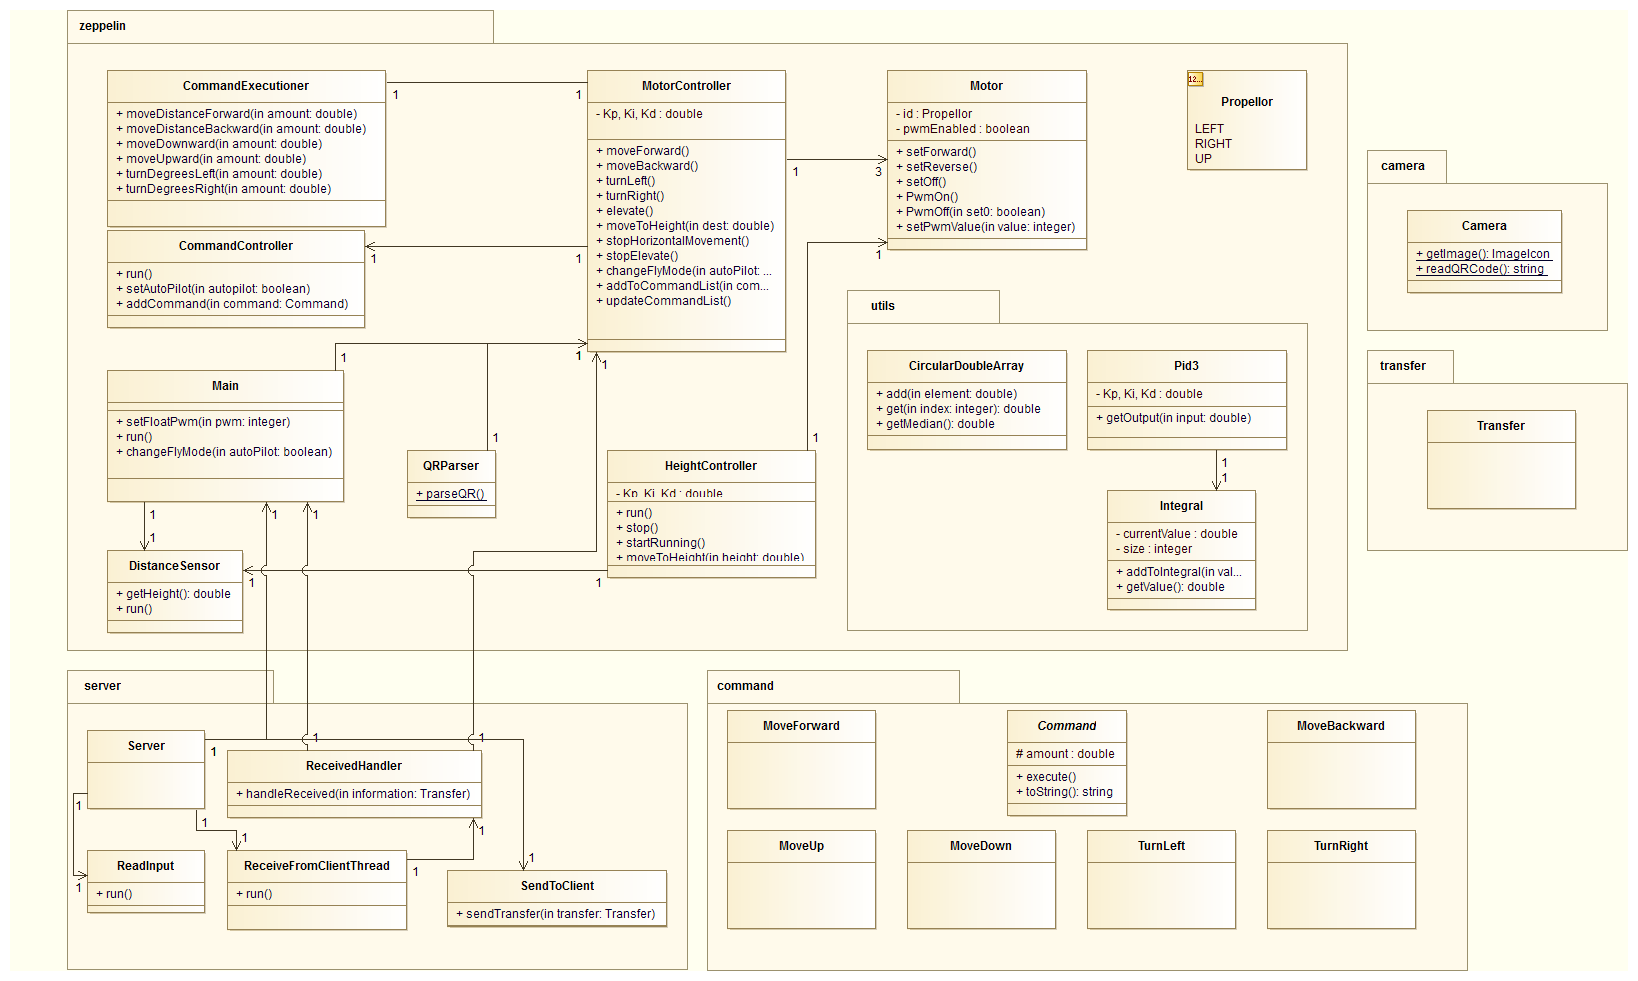
\includegraphics[scale=0.38,angle=90]{UML.png}
\caption{Klassediagram van de interne programmatie}
\label{UML}
\end{figure}

% == GUI == %
\section{GUI}
\begin{wrapfigure}{r}{0.45\textwidth}
\centering
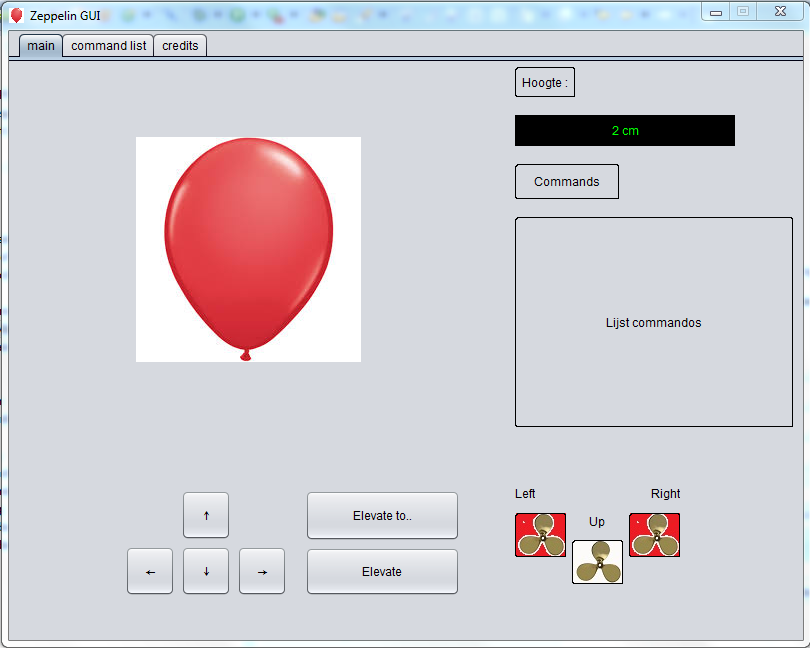
\includegraphics[width=0.43\textwidth]{GUI.png}
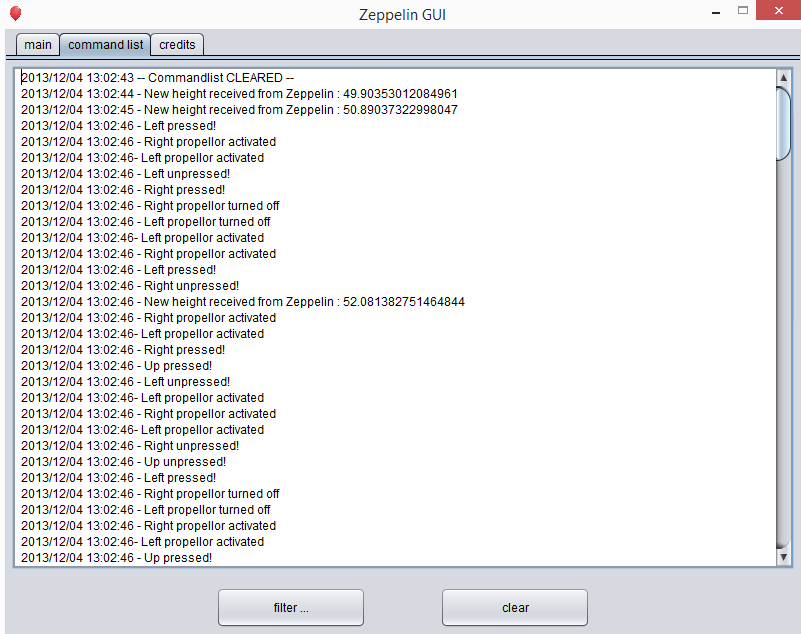
\includegraphics[width=0.43\textwidth]{GUI2.png}
\caption{GUI}
\label{GUI}
\end{wrapfigure}

De User Interface stelt de gebruiker in staat om vanaf een client-pc verbinding te maken met de zeppelin. De GUI geeft informatie weer over de status, zoals de huidige hoogte en commando's die worden uitgevoerd. Daarnaast kan de gebruiker de zeppelin aansturen via de pijltjestoetsen. \\

De eerste tab (`main') toont de huidige hoogte en de toestand van de propellers. Er is ruimte voorzien om foto's (van de camera) te tonen en om de commando's weer te geven die in de wachtrij van de zeppelin zitten. Verder zijn hier toetsen om de motoren aan te sturen en om de zeppelin naar een bepaalde hoogte te laten stijgen.\\

De tweede tab geeft een uitgebreider overzicht van de informatie die wordt uitgewisseld tussen de GUI en zeppelin, met een indicatie van de tijd. \\

De zeppelin (server) staat slechts toe dat er \'e\'en client verbindt en dat er dus maar \'e\'en GUI wordt getoond. Het zou mogelijk zijn meerdere clients toegang te geven, maar om conflicten (met pijltjestoetsen) te vermijden en om bandbreedte te besparen (bij het doorsturen van afbeeldingen), ondersteunt de server maar 1 client. \\




% == BESLUIT == %
\section{Besluit}
We zijn er in geslaagd het fysiek ontwerp van de zeppelin te bouwen en Java-software te schrijven die de Raspberry Pi aanstuurt. Via sockets wisselt de zeppelin informatie uit met een client en kan de zeppelin via de pijltjestoetsen worden aanstuurd. Verder toont de zeppelin op de GUI zijn status en afbeeldingen aan de gebruiker. \\

De zeppelin kan QR-codes lezen en de opdrachten hieruit interpreteren. De HeightController regelt op elk moment de hoogte door middel van een PID-algoritme. Om andere commando's uit te voeren moeten we vertrouwen op gegevens die de tijd dat een motor actief is, linken aan de afstand of hoek. Wel is het mogelijk om aan de hand van foto's van de camera de fout in afstand of draaihoek ten opzichte van een QR-code te bepalen, waardoor het in principe mogelijk is bij te sturen. \\



% == APPENDICES == %
\newpage\makeappendix

\section{Beschrijving van het proces}
\begin{itemize}
\item \textbf{Welke moeilijkheden heb je ondervonden tijdens de uitwerking?} \\
Kleine startproblemen bestonden uit het niet direct aanwezig zijn van alle hardware, waardoor we tijdens de beginfase veronderstellingen moesten maken over hoe deze in de praktijk zou werken. Hierdoor moesten we soms op enkele beslissingen terugkomen. De praktijk voldeed dus (zoals we wel hadden verwacht) niet volledig aan de theorie. Dit was goed duidelijk bij het naar links of rechts draaien van de zeppelin. In theorie zou deze op eenzelfde plaats moeten blijven hangen boven een bepaald punt, maar dit was niet het geval. \\
Een ander probleem dat we vooral in het begin hadden, was de communicatie tussen de zeppelin en de GUI. Dit is echter een probleem waarmee alle groepen te maken hadden. In feite waren we er vrij snel in geslaagd de communicatie te laten werken, maar in latere weken hebben we soms nog aanpassingen moeten maken omdat er problemen opdoken van zodra meer informatie werd verstuurd. \\
Een probleem waar we verschillende uren mee bezig zijn geweest, is de interferentie tussen de neerwaartse motor en de afstandssensor. Als de motor wordt ingeschakeld, vertoonden de meetwaarden van de afstandssensor deviant gedrag. Om dit op te lossen, gaan we het frame aanpassen. \\
Later hadden we een nieuw probleem waarbij de sensor een veel grotere hoogte gaf dan de werkelijke hoogte. Dit bleek veroorzaakt door de vele threads die op dat moment ge\"introduceerd waren. \\
\item \textbf{Welke lessen heb je getrokken uit de manier waarop je het project hebt aangepakt?} \\
Dat veel testen in de praktijk noodzakelijk zijn. Dit is uiteraard te verwachten, maar is op bepaalde momenten overduidelijk. Goede voorbeelden hiervan zijn de problemen met de distancesensor (hierboven beschreven) en het regelen van de hoogte van de zeppelin. Aannames die je maakt zijn vaak niet waar (bijvoorbeeld naar boven vliegen brengt vaak een horizontale beweging met zich mee), en dit wordt pas duidelijk wanneer je de zeppelin echt aan het werk ziet met de code. \\
Op het gebied van groepswerking was het naar de tussentijdse demo toe duidelijk dat er een vrij groot verschil zat op het aantal gepresteerde uren. We beseffen nu dat we van in het begin een goede taakverdeling moeten voorzien, en dat het belangrijk is deze elke week op te volgen en desnoods bij te sturen. \\
We hebben in dit project ook goed leren werken met threads en synchronizatie, een thema dat we voordien bijna alleen theoretisch hadden gezien. \\
Wat nogmaals duidelijk werd is het belang van goede documentatie, zeker voor uitgebreide klasses zoals de GUI. Dit is iets waar we vanaf het begin rekening mee hebben gehouden. \\
Op het vlak van rapporteren hebben we vooral geleerd dat we veel moeten motiveren. We mogen ook niet verwachten dat de lezer even goed als wijzelf op de hoogte is van de details van het project.
\item \textbf{Hoe verliep het werken in team? Op welke manier werd de teamco\"ordinatie en planning aangepakt?} \\
Naar de tussentijdse demo toe was het duidelijk dat onze taakverdeling niet perfect was, waardoor de gewerkte uren vrij sterk uit elkaar lagen. Sommige taken waren snel afgewerkt, en er was soms niet genoeg werk voor iedereen waardoor er af en toe met 2-3 personen aan 1 computer gewerkt moest worden. \\
De weken nadien hebben we ons best gedaan om ervoor te zorgen dat degenen die achter liepen in aantal uren, wat meer taken kregen. \\
Wanneer we met de volledige groep samenkomen, is het voordeel dat iedereen zijn mening kan geven en kan bijdragen aan het project. Het nadeel is echter dat we nooit alle vijf gedurende de hele sessie aan maximale productiviteit kunnen werken. \\
De communicatie tussen de verschillende groepsleden verliep vlot en bij problemen konden we terecht op de Facebook-groep die we voor dit project hebben aangemaakt. \\
De eerste les hebben we een teamco\"ordinator en secretaris gekozen, maar deze keuzes waren eerder gemaakt omdat we toen nog geen idee hadden hoe het project ging verlopen. Uiteindelijk hebben we allemaal gedeeltelijk de rol van secretaris ingevuld: wie even geen taak had, kon aan de verslagen werken, die dan nadien door alle groepsleden nagelezen en aangepast werden. \\ 
Tijdens de eerste 2 lessen werd het al duidelijk welke grote delen er geprogrammeerd moesten worden. Hiervoor hebben we dan een aantal personen per deel gezet.  Meer hierover is in het volgende deel terug te vinden.

\end{itemize}


\section{Beschrijving van de werkverdeling}
De eerste lessen hebben we besloten dat er 3 grote delen waren die moesten afgewerkt worden: de GUI, de communicatie tussen GUI en zeppelin en de zeppelin zelf. Ook waren er de tussentijdse verslagen en het testen van de onderdelen. \\
\begin{itemize}
\item Wander Bavin: Heeft meegewerkt aan het onderdeel GUI. Dit deel vroeg vooral in het begin wat werk. Nadat de GUI afgewerkt was heeft hij verslagen gemaakt/nagelezen en uiteindelijk meegewerkt aan het motor-gedeelte. Indien er extra informatie op de GUI moest verschijnen heeft hij hiervoor gezorgd. Vervulde de rol van co\"ordinator.
\item Dimitri Jonckers: Heeft meegewerkt aan het onderdeel GUI. Heeft net zoals Wander de verslagen gemaakt en nagelezen, alsook meegewerkt aan de interne programmatie van de Raspberry Pi. Ook hij heeft de GUI aangepast wanneer nodig, en het UML-diagram opgesteld. Heeft thuis veel opzoekwerk gedaan/geprogrammeerd. Heeft de meeste weekly progress reports geschreven.
\item Sunil Tandan: Heeft gewerkt aan het deel communicatie tussen GUI en zeppelin. Dit was een groot en belangrijk deel dat hij op zichzelf heeft gemaakt. Dit deel vroeg redelijk wat werk en moest elke keer wel een beetje aangepast worden (bijvoorbeeld voor het versturen van images). Heeft elk verslag nagelezen en delen over de communicatie toegevoegd. Nadien heeft hij het werken met de camera op zich genomen.
\item Wout Vekemans: Heeft meegewerkt aan het deel motoren/zeppelin. Tijdens de beginfase voornamelijk verslagen gemaakt/nagelezen. Heeft samen met Vince de afstandssensor getest/geprogrammeerd en is daarna aan de motoren beginnen werken. Hij vervulde de rol van secretaris en stuurde de verslagen dus telkens door.
\item Vince Goossens: Heeft meegewerkt aan het deel motoren/zeppelin. Tijdens de beginfase voornamelijk verslagen nagelezen. Heeft samen met Wout de afstandssensor getest/geprogrammeerd en is daarna aan de motoren beginnen werken/programmeren.
\end{itemize}

Na de tussentijdse demo is iedereen gedeeltelijk bezig geweest met het testen van de camera en de motoren, en bezig geweest met het implementeren van de commando's.

Hieronder is een tabel te vinden met de gewerkte uren binnen en buiten de sessies: \\

TODO aanvullen en updaten

\begin{tabular}{r||r|r|r|r|r}
Overzicht: & Dimitri Jonckers & Wander Bavin & Wout Vekemans & Sunil Tandan & Vince Goossens \\
\hline \hline 
30/09 - 06/10 & 5 & 5 & 5 & 7 & 5 \\
07/10 - 13/10 & 15.5 & 12 & 6 & 11 & 5 \\
14/10 - 20/10 & 11 & 10.5 & 6.75 & 9 & 6.25 \\
21/10 - 27/10 & 9 & 5.5 & 6 & 9 & 5.5 \\
28/11 - 03/11 & 12 & 5 & 5 & 5 & 5 \\
04/11 - 10/11 & 15 & 16 & 10 & 16.5 & 10 \\
11/11 - 17/11 & 17 & 14.5 & 8 & 18.5 & 10 \\
18/11 - 24/11 & 9.5 & 15 & 9 & 9 & 9 \\
18/11 - 24/11 & 11.5 & 5 & 11 & 13 & 11 \\
\hline \hline
Totaal &  &  &  &  &  \\
\end{tabular}

\section{Kritische analyse}
De groepssfeer was goed. De werkverdeling kon echter wel beter. In de periode voor de tussentijdse demo wou iedereen wel ergens aan werken, maar vaak was iemand anders hiermee al begonnen. We zouden beter (en vanaf het begin) moeten zorgen voor een goede taakverdeling en deze ook opvolgen en aanpassen aan de hand van eventuele problemen en van verschillen in werkuren. \\
Een tweede punt van kritiek is dat in de loop van het project een gedeelte van de code van de zeppelin sterk uitgebreid is. Hierdoor is de code niet altijd even duidelijk meer (bijvoorbeeld de introductie van een aantal boolean-variabelen om de flow te regelen). Dit betekent dat er extra aandacht nodig is bij het aanpassen van de code. In principe is het mogelijk deze code op te kuisen, maar we hebben ons in code laatste weken voor de demo vooral moeten bezighouden met het toevoegen van nieuwe functionaliteit. \\
Over de kwaliteit van de code zelf zijn we wel tevreden. Omwille van problemen met het aantal threads zijn we verplicht geweest deze een stuk effici\"enter te maken. De meeste delen van de code zijn uitgebreid gedocumenteerd. \\
Verder is het fysiek ontwerp van onze zeppelin niet perfect. Idealiter hadden we een nieuw frame moeten laten maken, waarbij een deftige plaats voor de distancesensor voorzien is en dat gemaakt is uit een stevig materiaal zoals plexiglas. Omwille van het vele werk met de programmatie zijn we hier niet toe gekomen. \\
We zijn tevreden over onze keuze voor Java en hebben eigenlijk op geen enkel moment tijdens het project gedacht dat we beter af zouden zijn door Python te gebruiken. Alle functionaliteit die we moesten implementeren, was zonder problemen mogelijk in Java. \\

\end{document}
